\documentclass[slug=PET, room=Andreas-Schubert-Bau\,\ K\ 1A, supervisor=Anne-Sophie\ Berthold, coursedate=13.\ 12.\ 2019]{../../Lab_Report_LaTeX/lab_report}

\title{Postitronenemissionstomographie}
\author{Oliver Matthes, Valentin Boettcher}
\usepackage{todonotes}
\graphicspath{ {figs/} }
\usepackage{tikz}
\usepackage{pgf}
\usepackage[version=4]{mhchem}
\usepackage[ngerman]{babel}
\usepackage{subcaption}
\usepackage{amssymb}

% bib
\addbibresource{protokoll.bib}

\begin{document}
\maketitle

\section{Auswertung}
\label{sec:ausw}

\subsection{Theoriebeispiel}
\label{sec:theobei}
Zur Verbesserung des verst\"andnisses der Projektions- und
Rekonstruktionsprozesse, werden diese hier anhand eines einfachen
Beispiels nachvollzogen.

\begin{figure}[htp]
  \centering
  \begin{subfigure}[t]{.25\textwidth}
    \centering
    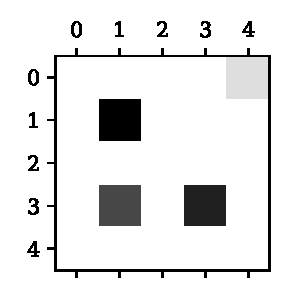
\includegraphics[width=.6\textwidth]{../auswertung/figs/theory/source.pdf}
    \caption{Ausgangsmatrix}
    \label{fig:theory-source}
  \end{subfigure}
  \begin{subfigure}[t]{.25\textwidth}
    \centering
    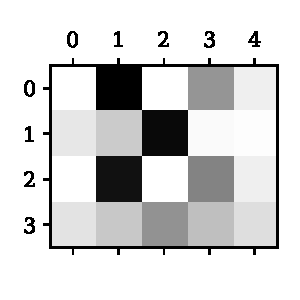
\includegraphics[width=.6\textwidth]{../auswertung/figs/theory/projection.pdf}
    \caption{Sinogram}
    \label{fig:theory-projection}
  \end{subfigure}
  \begin{subfigure}[t]{.25\textwidth}
    \centering
    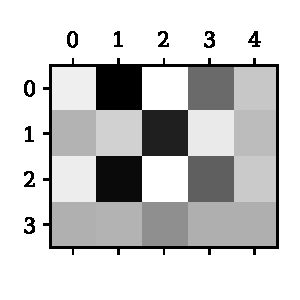
\includegraphics[width=.6\textwidth]{../auswertung/figs/theory/convoluted.pdf}
    \caption{Gefiltertes Sinogram}
    \label{fig:theory-convoluted}
  \end{subfigure}
  \begin{subfigure}[t]{.25\textwidth}
    \centering
    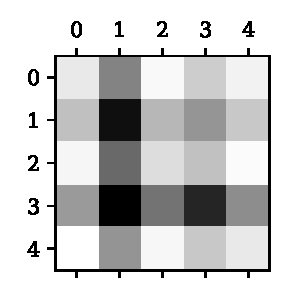
\includegraphics[width=.6\textwidth]{../auswertung/figs/theory/rec_simple.pdf}
    \caption{Einfache R\"uckprojektion}
    \label{fig:theory-rec_simple}
  \end{subfigure}
  \begin{subfigure}[t]{.25\textwidth}
    \centering
    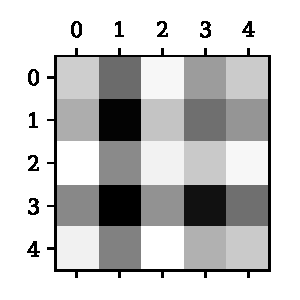
\includegraphics[width=.6\textwidth]{../auswertung/figs/theory/rec_filtered.pdf}
    \caption{Gefilterte R\"uckprojektion}
    \label{fig:theory-rec_filtered}
  \end{subfigure}
  \caption[Graustufendarstellung der
  Beispielmatrizen]{Graustufendarstellung der Matrizen aus den
    Teilschritten des Beispiels. Es wurden jeweils die Matrixelemente
    in das Interval \([0,1]\) reskaliert.}
  \label{fig:graubei}
\end{figure}

Im ersten Schritt wird die Projektion~\ref{fig:theory-projection} des
Ausgangsbildes~\ref{fig:theory-source} aus Verschiedenen Winkeln
berechenet. Dabei wurden die diagonalen entsprechend gewichtet.

\begin{equation}
  \label{eq:proj}
  \mathfrak{M}_0 =
  \begin{pmatrix}
    0 & 0 & 0 & 0 & 2\\
    0 & 9 & 0 & 0 & 0\\
    0 & 0 & 0 & 0 & 0\\
    0 & 7 & 0 & 8 & 0\\
    0 & 0 & 0 & 0 & 0\\
  \end{pmatrix}
  \implies
  \left(
    \begin{array}{ccccc|c}
      0. & 16. & 0. & 8. & 2 & 0^\circ\\
      2.73 & 4.95 & 15.47 & 0.68 & 0.28 & 45^\circ\\
      0. & 15. & 0. & 9. & 2. & 90^\circ\\
      3.12 & 5.24 & 8.19 & 5.85 & 3.51 & 135^\circ\\
    \end{array}\right) = \mathfrak{P}_0
\end{equation}

Ein gefiltertes Sinogram~\ref{fig:theory-convoluted} ergibt sich durch
Faltung der Zeilen von \(\mathfrak{M}_0\) mit
\(F = \mqty(-.1 & .25 & -.1)\).

\begin{equation}
  \label{eq:filter}
  \mathfrak{M}_1 = \mathfrak{M}_0 * F =
  \begin{pmatrix}
    -1.6 & 4. & -2.4 & 1.8 & -0.3\\
    0.188 & -0.583 & 3.304 & -1.405 & 0.002\\
    -1.5 & 3.75 & -2.4 & 2.05 & -0.4\\
    0.256 & 0.179 & 0.938 & 0.293 & 0.292\\
  \end{pmatrix}
\end{equation}

Die R\"uckprojektion des Einfachen sinogramms
ergib~\ref{fig:theory-rec_simple}.

{\footnotesize
\setlength{\arraycolsep}{2.5pt}

\begin{align}
  \label{eq:simplerepr}
  \overbrace{\begin{pmatrix}
      0. & 16. & 0. & 8. & 2.\\
      0. & 16. & 0. & 8. & 2.\\
      0. & 16. & 0. & 8. & 2.\\
      0. & 16. & 0. & 8. & 2.\\
      0. & 16. & 0. & 8. & 2.\\
    \end{pmatrix}}^{0^\circ} & + \frac{1}{2}\overbrace{\begin{pmatrix}
      15.864 & 8.408 & 0.837 & 0.287 & 0.076\\
      12.636 & 15.864 & 8.408 & 0.837 & 0.287\\
      6.569 & 12.636 & 15.864 & 8.408 & 0.837\\
      2.78 & 6.569 & 12.636 & 15.864 & 8.408\\
      0.737 & 2.78 & 6.569 & 12.636 & 15.864\\
    \end{pmatrix}}^{45^\circ} \nonumber \\ + \overbrace{\begin{pmatrix}
      2. & 2. & 2. & 2. & 2.\\
      9. & 9. & 9. & 9. & 9.\\
      0. & 0. & 0. & 0. & 0.\\
      15. & 15. & 15. & 15. & 15.\\
      0. & 0. & 0. & 0. & 0.\\
    \end{pmatrix}}^{90^\circ} &+ \frac{1}{2}\overbrace{\begin{pmatrix}
      0.842 & 3.172 & 7.12 & 9.283 & 8.966\\
      3.172 & 7.12 & 9.283 & 8.966 & 9.886\\
      7.12 & 9.283 & 8.966 & 9.886 & 8.003\\
      9.283 & 8.966 & 9.886 & 8.003 & 3.569\\
      8.966 & 9.886 & 8.003 & 3.569 & 0.948\\
    \end{pmatrix}}^{135^\circ}\nonumber \\
  & = \begin{pmatrix}
    10.353 & 23.79 & 5.978 & 14.785 & 8.521\\
    16.904 & 36.492 & 17.845 & 21.902 & 16.087\\
    6.844 & 26.959 & 12.415 & 17.147 & 6.42\\
    21.031 & 38.768 & 26.261 & 34.933 & 22.988\\
    4.852 & 22.333 & 7.286 & 16.102 & 10.406\\
  \end{pmatrix} = \mathfrak{M}_1
\end{align}}

Aus dem gefilterten Sinogram ergibt sich auf \"ahnliche
Weise~\ref{fig:theory-rec_filtered}
{\footnotesize
\setlength{\arraycolsep}{2.5pt}

\begin{align}
  \label{eq:simplerepr}
  \overbrace{\begin{pmatrix}
      -1.6 & 4. & -2.4 & 1.8 & -0.3\\
      -1.6 & 4. & -2.4 & 1.8 & -0.3\\
      -1.6 & 4. & -2.4 & 1.8 & -0.3\\
      -1.6 & 4. & -2.4 & 1.8 & -0.3\\
      -1.6 & 4. & -2.4 & 1.8 & -0.3\\
    \end{pmatrix}}^{0^\circ} & + \frac{1}{2}\overbrace{\begin{pmatrix}
      3.165 & 0.261 & -1.305 & -0.012 & 0.001\\
      1.076 & 3.165 & 0.261 & -1.305 & -0.012\\
      -0.407 & 1.076 & 3.165 & 0.261 & -1.305\\
      0.182 & -0.407 & 1.076 & 3.165 & 0.261\\
      0.051 & 0.182 & -0.407 & 1.076 & 3.165\\
    \end{pmatrix}}^{45^\circ} \nonumber \\ +
  \overbrace{\begin{pmatrix}
      -0.4 & -0.4 & -0.4 & -0.4 & -0.4\\
      2.05 & 2.05 & 2.05 & 2.05 & 2.05\\
      -2.4 & -2.4 & -2.4 & -2.4 & -2.4\\
      3.75 & 3.75 & 3.75 & 3.75 & 3.75\\
      -1.5 & -1.5 & -1.5 & -1.5 & -1.5\\
    \end{pmatrix}}^{90^\circ} &+ \frac{1}{2}\overbrace{\begin{pmatrix}
      0.069 & 0.258 & 0.351 & 0.646 & 0.972\\
      0.258 & 0.351 & 0.646 & 0.972 & 0.759\\
      0.351 & 0.646 & 0.972 & 0.759 & 0.486\\
      0.646 & 0.972 & 0.759 & 0.486 & 0.295\\
      0.972 & 0.759 & 0.486 & 0.295 & 0.079\\
    \end{pmatrix}}^{135^\circ}\nonumber \\
           &= \begin{pmatrix}
             -0.383 & 3.86 & -3.277 & 1.717 & -0.214\\
             1.117 & 7.808 & 0.104 & 3.683 & 2.123\\
             -4.028 & 2.461 & -2.732 & -0.09 & -3.11\\
             2.564 & 8.032 & 2.267 & 7.375 & 3.728\\
             -2.589 & 2.97 & -3.861 & 0.985 & -0.178\\
           \end{pmatrix} = \mathfrak{M}_2
\end{align}
}

Es ist zu erkennen, das in beiden rekonstruktionen die starken Signale
\((1,1),\,(3,1),\,(3,3)\) klar zu identifizerien, wenngleich die
Unterschiede in der signalst\"arke nicht im urspr\"unglichen
Verh\"altniss stehen. Die gefilterte R\"uckprojektion weist in den
Randfeldern und im Mittleren Feld einen h\"oheren Kontrast auf,
erzeugt aber dennoch nur ein geringf\"ugig besseres und in manchen
Bereichen (Ecken) sogar ein schlechteres Bild. Das schwache Signal
\((0,4)\) wurde in beiden F\"allen nicht rekonstruiert. F\"uhrt man
die Rechnung ohne diesen Punkt aus, ergibt sich kaum ein
Unterschied. Schwache Signale werden also nicht gut reproduziert.

\newpage
\section{Verzeichnisse}
\label{sec:literatur}

\listoffigures

\listoftables

\printbibliography
\end{document}
